\documentclass[a4paper, 11pt]{article}
\usepackage[top=3cm, bottom=3cm, left=2cm, right=2cm]{geometry} 
\geometry{a4paper} 
\usepackage[utf8]{inputenc}
\usepackage[vietnamese]{babel}
\usepackage{xcolor}
\usepackage{sectsty}
\usepackage{textcomp}
\usepackage{graphicx} 
\usepackage{amsmath,amssymb}
\usepackage{algorithm,algcompatible}
\usepackage{caption}
\usepackage{subcaption}
\usepackage{bm}
\usepackage{tikz}
\usepackage{multirow, multicol, makecell}
\usepackage{longtable}
\usepackage{enumitem}
\setlist[itemize]{leftmargin=*}
\usepackage[pdftex,bookmarks,colorlinks,breaklinks]{hyperref}  
%\hypersetup{linkcolor=black,citecolor=black,filecolor=black,urlcolor=black} % black links, for printed output
\usepackage{memhfixc}
\usepackage{wrapfig}
\usepackage{pdfsync}  
\usepackage{fancyhdr}
\usepackage{pifont}
\usepackage{listings}
\usepackage{lstfiracode}
\lstset{style=FiraCodeStyle,basicstyle=\ttfamily,columns=fullflexible,breaklines=true,commentstyle=\color{green},
keywordstyle=\color{magenta},
numberstyle=\color{gray},
stringstyle=\color{red}}
\makeatletter
\def\lst@visiblespace{ }
\makeatother
\usepackage[export]{adjustbox}

\pagestyle{fancy}
\sloppy

\graphicspath{ {images/} }
\setlength{\headheight}{16.50983pt}
\setlength{\parindent}{0pt}

\newenvironment{vnalgorithm}[1][]
  {\begin{algorithm}[#1]
     \selectlanguage{vietnamese}%
     \floatname{algorithm}{Thuật toán}%
     \algnewcommand\INPUT{\item[\textbf{Đầu vào:}]}%
     \algnewcommand\OUTPUT{\item[\textbf{Đầu ra:}]}%
     \algnewcommand\BEGIN{\item[\textbf{begin}]} %
     \algnewcommand\DO{\textbf{ do}} %
     \algnewcommand\RETURN{\State\textbf{return }}%
     \algnewcommand\BREAK{\State\textbf{break}}%
     \algnewcommand\CONTINUE{\State\textbf{continue}}
     \algnewcommand\END{\item[\textbf{end}]}%
     % Set other language requirements
  }
  {\end{algorithm}}


\title{\textbf{Bài tập Thực hành Nhập môn Trí tuệ Nhân tạo tuần 4}}
\author{Nguyễn Lê Ngọc Duy - 20280023 - 20KDL1}
\date{}

\begin{document}
\maketitle
\hypersetup{linkcolor=black}
\tableofcontents
\clearpage

\section{Giới thiệu bài toán.}
Trong tuần này chúng ta sẽ vận dụng tất cả các thuật toán tìm kiếm đã được tìm hiểu ở các tuần trước để giải quyết bài toán được đặt ra trong tuần này như sau: Tìm đường đi ngắn nhất từ điểm xuất phát là điểm $S$ tới điểm kết thúc là điểm $G$ trong mặt phẳng hai chiều với các chướng ngại vật là các đa giác lồi như hình 1.

\begin{figure}[h]
  \centering
  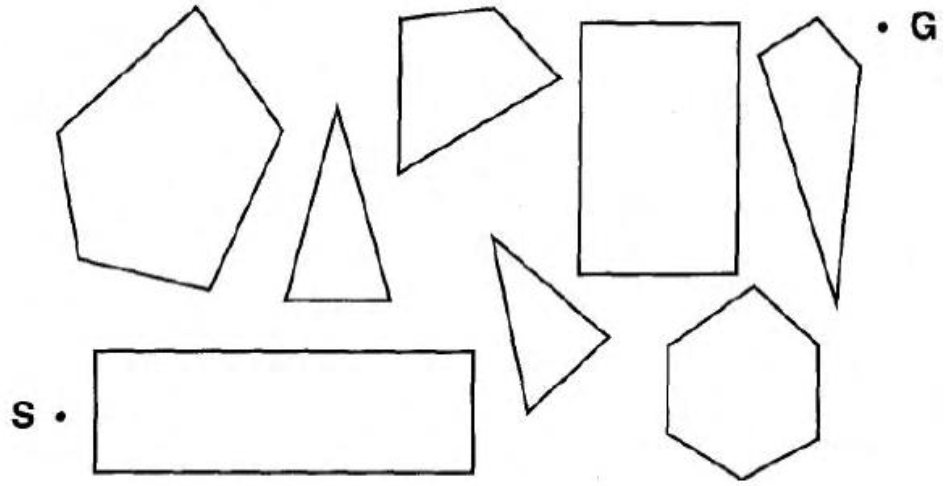
\includegraphics[width=\textwidth,height=\textheight,keepaspectratio]{problem.png}
  \caption{Hình vẽ mô tả bài toán}
\end{figure}
Trước khi tiến hành giải bài toán, ta cần nhắc lại các thuật toán tìm kiếm đã được chúng ta tìm hiểu ở các tuần trước đó.

\section{Các giải thuật tìm kiếm.}
Ở phần này, chúng ta sẽ chỉ nhắc lại mã giả của các giải thuật tìm kiêm đã được tìm hiểu ở các tuần trước đó (xem các thuật toán từ 1 đến 5).

\begin{vnalgorithm}
  \caption{Thuật toán Depth First Search - DFS}
  \begin{algorithmic}[1]
      \INPUT{đồ thị $G$, node xuất phát $start$, node kết thúc $end$.}
      \OUTPUT{đường đi từ $start$ đến $end$}
      \BEGIN
          \STATE{Khởi tạo danh sách $L$ chứa trạng thái ban đầu.}
          \WHILE{true}
              \IF{$L$ rỗng}
                  \STATE{Thông báo không có đường đi.}
                  \BREAK
              \ENDIF
          \ENDWHILE
          \STATE{Loại trạng thái $u$ ở đầu danh sách $L$.}
          \IF{$u$ là trạng thái kết thúc}
              \RETURN{đường đi từ $start$ đến $u$.}
          \ENDIF
          \STATE{Lấy các trạng thái $v$ kề với $u$ và thêm vào đầu danh sách $L$.}
          \FOR{mỗi trạng thái $v$ kề với $u$}
              \STATE{$father(v) = u$}
          \ENDFOR
      \END
  \end{algorithmic}
\end{vnalgorithm}

\begin{vnalgorithm}
  \caption{Thuật toán Breath First Search - BFS}
  \begin{algorithmic}[1]
      \INPUT{đồ thị $G$, node xuất phát $start$, node kết thúc $end$.}
      \OUTPUT{đường đi từ $start$ đến $end$}
      \BEGIN
          \STATE{Khởi tạo danh sách $L$ chứa trạng thái ban đầu.}
          \WHILE{true}
              \IF{$L$ rỗng}
                  \STATE{Thông báo không có đường đi.}
                  \BREAK
              \ENDIF
          \ENDWHILE
          \STATE{Loại trạng thái $u$ ở đầu danh sách $L$.}
          \IF{$u$ là trạng thái kết thúc}
              \RETURN{đường đi từ $start$ đến $u$.}
          \ENDIF
          \STATE{Lấy các trạng thái $v$ kề với $u$ và thêm vào cuối danh sách $L$.}
          \FOR{mỗi trạng thái $v$ kề với $u$}
              \STATE{$father(v) = u;$}
          \ENDFOR
      \END
  \end{algorithmic}
\end{vnalgorithm}

\begin{vnalgorithm}
  \caption{Thuật toán Uniform Cost Search - UCS}
  \begin{algorithmic}[1]
      \INPUT{đồ thị $G$, node xuất phát $start$, node kết thúc $end$.}
      \OUTPUT{đường đi từ $start$ đến $end$ và chi phí của đường đi}
      \BEGIN
          \STATE{Tạo hàng đợi ưu tiên rỗng $NganChua$.}
          \STATE{Thêm nút $start$ vào $NganChua$.}
          \LOOP
              \IF{$NganChua$ rỗng}
                  \RETURN{không tồn tại đường đi.}
              \ELSE
                  \STATE{$Nut$ = TimChiPhiNhoNhat($NganChua$) }
                  \IF{KiemTraCauHoiDich($BaiToan$) trên TrangThai($Nut$) đúng}
                      \RETURN LoiGiai($Nut$)
                  \ENDIF
              \ENDIF
          \ENDLOOP
          \STATE {$LoiGiai$ = Mo($Nut$, $BaiToan$)}
          \STATE {$NganChua$ = ThemTatCa($LoiGiai$, $NganChua$)}
      \END
  \end{algorithmic}
\end{vnalgorithm}

\begin{vnalgorithm}
  \caption{Thuật toán Greedy Best First Search (GBFS)}
  \begin{algorithmic}[1]
    \INPUT Bài toán.
    \OUTPUT Lời giải hoặc thông báo: Không tồn tại lời giải.
    \STATE {\lstinline|insert(state = initial_state, priority = 0)| \lstinline|into search.queue|;}
    \WHILE{\lstinline|search.queue not empty|}
      \STATE {\lstinline|current_queue.entry = pop item from front of search.queue|}
      \STATE {\lstinline|current_state = current_queue.entry.state|;}
      \STATE {\lstinline|current_heuristic = current_queue.entry.heuristic|;}
      \STATE {\lstinline|starting_counter = counter from current_queue.entry|;}
      \STATE {\lstinline|applicable_actions = array of actions applicable in current_state|;}
      \FOR {\textbf{all} \lstinline|index ?i in applicable_actions >= | \lstinline| starting_counter|}
        \STATE \lstinline|current_action = applicable_actions[?i];|
        \STATE \lstinline|successor_state = current_state.apply(current_action);|
        \IF{\lstinline{successor_state is goal state}}
          \RETURN{\lstinline|solution_path|;}
        \ENDIF
        \STATE{\lstinline|successor_heuristic = heuristic value of successor_state|;}
        \IF{\lstinline{successor_heuristic < current_heuristic}}
          \STATE {\lstinline|insert(current_state, current_heuristic, ?i + 1)| \lstinline|to search.queue|;}
          \STATE {\lstinline|insert(successor_state, successor_heuristic, 0)| \lstinline|to search.queue|;}
          \STATE \textbf{break for;}
        \ELSE
          \STATE {\lstinline|insert(successor_state, successor_heuristic, 0)| \lstinline|to search.queue|;}
        \ENDIF
      \ENDFOR
    \ENDWHILE
  \end{algorithmic}
\end{vnalgorithm}

\begin{vnalgorithm}
  \caption{Thuật toán A*}
  \begin{algorithmic}[1]
    \INPUT Bài toán.
    \OUTPUT Lời giải hoặc thông báo: Không tồn tại lời giải.
    \STATE {$\text{OPEN} = T_0$}
    \STATE {$g(T_0) = 0, h(T_0) = 0, f(T_0) = 0$}
    \STATE {$\text{CLOSE} = \emptyset$}
    \LOOP
      \IF{$\text{OPEN}$ rỗng}
        \STATE {Bài toán vô nghiệm.}
        \STATE \textbf{exit}
      \ELSE
        \STATE {Lấy $T_{\text{max}}$ ra khỏi OPEN}
        \STATE {Đưa $T_{\text{max}}$ vào CLOSE}
        \IF{$T_{\text{max}}$ là trạng thái đích}
          \STATE{Lời giải là $T_{\text{max}}$}
          \STATE \textbf{exit}
        \ELSE
          \STATE {Tạo danh sách tất cả các trạng thái kế tiếp $T_K$ của $T_{\text{max}}$}
          \FOR {\textbf{each} $T_K$}
            \STATE {$g(T_K) = g(T_{\text{max}}) + \text{cost}(T_{\text{max}}, T_K)$}
            \IF{tồn tại $T_{K'}$ trong OPEN trùng với $T_K$}
              \IF{$g(T_K) < g(T_{K'})$}
                \STATE {$g(T_{K'}) = g(T_K)$}
                \STATE {Tính lại $f(T_{K'})$}
                \STATE {FATHER($T_{K'}$) = $T_{\text{max}}$}
              \ENDIF
            \ENDIF
            \IF{tồn tại $T_{K'}$ trong CLOSE trùng với $T_K$}
              \IF{$g(T_K) < g(T_{K'})$}
                \STATE {$g(T_{K'}) = g(T_K)$}
                \STATE {Tính lại $f(T_{K'})$}
                \STATE {FATHER($T_{K'}$) = $T_{\text{max}}$}
              \ENDIF
            \ENDIF
            \STATE{\textit{Lan truyền} sự thay đổi của $f$ và $g$ cho tất cả các trạng thái kế tiếp của $T_i$ (ở tất cả các cấp) đã được lưu trữ trong CLOSE và OPEN.}
            \IF{$T_K$ chưa xuất hiện trong cả OPEN và CLOSE}
              \STATE{Thêm $T_K$ vào OPEN}
              \STATE{$f(T_K) = g(T_K) + h(T_K)$}
            \ENDIF
          \ENDFOR
        \ENDIF  
      \ENDIF
    \ENDLOOP
  \end{algorithmic}
\end{vnalgorithm}

\clearpage

\section{Giải bài toán.}

\subsection{Trả lời câu hỏi 1a.}
Ta có thể định nghĩa lại bài toán như sau: Cho một không gian $W = {\mathbb{R}}^2$ và một tập hợp hữu hạn các đa giác lồi (cũng chính là các chướng ngại vật $O$), mục tiêu của chúng ta là di chuyển tác nhân (được biểu diễn bởi một điểm) từ vị trí ban đầu $(x_s, y_s)$ tới vị trí kết thúc $(x_g, y_g)$ sao cho đường đi dược tạo thành là ngắn nhất có thể và đường đi đó phải đi qua những khoảng trống, định nghĩa bởi không gian $F = W - O$, hay nói cách khác, tác nhân không thể di chuyển qua các đa giác lồi $O$.

Khi đó tập không gian trạng thái của chúng ta chính là tất cả các vị trí $(x, y) \in {\mathbb{R}}^2$ nằm trong không gian $F$. Do số lượng các chướng ngại vật là hữu hạn, cho nên ta chỉ ra được sự tồn tại của không gian $F$ này. Trong không gian ${\mathbb{R}}^2$, số lượng các điểm $(x, y)$ nằm trong này là vô hạn, do đó số lượng các điểm trong không gian $F$ cũng là vô hạn (tuy nhiên số lượng các điểm này không nhiều hơn số lượng các điểm trong không gian ${\mathbb{R}}^2$). 

Có rất nhiều đường đi từ vị trí ban đầu $(x_s, y_s)$ tới vị trí kết thúc $(x_g, y_g)$, nhưng chỉ có một đường đi tối ưu được hình thành bởi tập hợp các đỉnh thuộc các đa giác chướng ngại vật và 2 cạnh nối 2 đầu của dường gấp khúc này đến lần lượt đỉnh đầu và đỉnh cuối của đường đi tối ưu.

\subsection{Trả lời câu hỏi 1b.}
Trước khi trả lời câu hỏi này, ta cần định nghĩa đường đi ngắn nhất Eucildean: Đường đi ngắn nhất từ một đỉnh $p$ nằm trên đa giác đến đỉnh $q$ bất kì nào khác được biểu diễn bởi $\rho = \langle p, p_1, p_2, \cdots, p_k, q \rangle$, trong đó mỗi đỉnh $p_1, p_2, \cdots, p_k$ là một đỉnh của một đa giác. (*)

Ta cần chứng minh rằng nhận định trên (cũng chính là ý của câu hỏi 1b) là dúng. Để chứng minh nhận định này, ta sẽ dùng phương pháp phản chứng. Đầu tiên, ta giả sử rằng có ít nhất một đỉnh $p_i$ nào đó trong đường đi ngắn nhất \textit{không} là đỉnh của đa giác. Ta xét các đỉnh từng đôi một không thẳng hàng, nghĩa là 3 đỉnh bất kì luôn tạo thành một tam giác.

Ta chia thành 3 trường hợp như hình 2:

\begin{figure}[h]
  \centering
  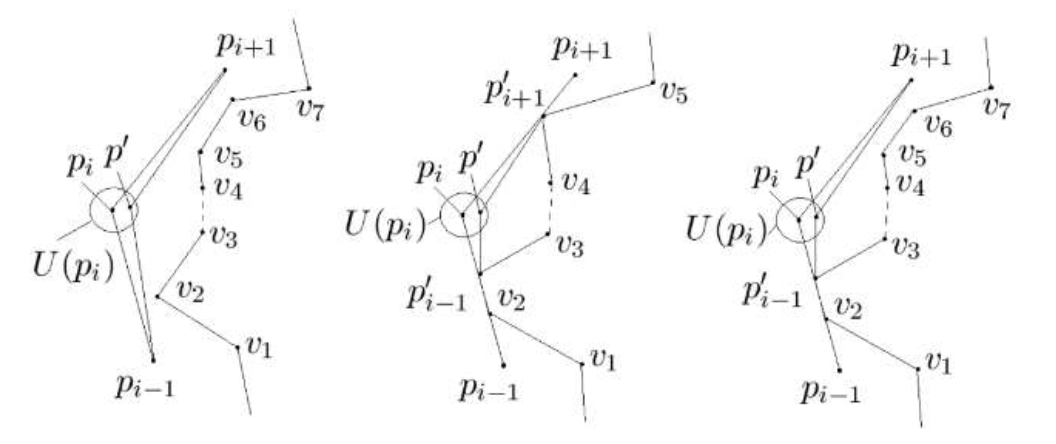
\includegraphics[width=\textwidth,height=\textheight,keepaspectratio]{proof.png}
  \caption{Minh hoạ ba trường hợp cần chứng minh}
\end{figure}


\begin{itemize}
  \item \textbf{Trường hợp 1: Cả hai cạnh $p_{i-1}p_i$ và $p_ip_{i+1}$ đều không là tiếp tuyến của đa giác hay không tiếp xúc với bất cứ đỉnh nào của đa giác.}\\
  Dựa vào hình vẽ, tồn tại một vùng nhỏ $U$ quanh $p_i$ sao cho tồn tại một điểm $p_i' \in U$ thoả mãn 
  \begin{equation}
    d(p_{i-1}, p_i') + d(p_i', p_{i+1}) < d(p_{i-1}, p_i) + d(p_i, p_{i+1})
  \end{equation}
  Suy ra nếu ta thay $p_i$ bởi $p_i'$, ta có thể thu dược một đường đi ngắn hơn, mâu thuẫn với giả sử $\rho$ là đường đi ngắn nhất.

  \item \textbf{Trường hợp 2: Cả hai cạnh $p_{i-1}p_i$ và $p_ip_{i+1}$ đều nằm trên cạnh của đa giác hay tiếp xúc với bất cứ đỉnh nào của đa giác.}\\
  Xét 2 đỉnh $p_{i-1}'$ và $p_{i+1}'$ gần nhất sao cho $p_{i - 1}'p_i$ và $p_ip_{i+1}'$ là tiếp tuyến của đa giác. Tương tự \textbf{Trường hợp 1}, ta có thể tìm được một điểm $p_i'$ sao cho
  \begin{equation}
    d(p_{i-1}, p_i') + d(p_i', p_{i+1}) < d(p_{i-1}, p_i) + d(p_i, p_{i+1})
  \end{equation}
  Điều này mâu thuẫn với giả sử $\rho$ là đường đi ngắn nhất.

  \item \textbf{Trường hợp 3: Trong hai cạnh $p_{i-1}p_i$ và $p_ip_{i+1}$ chỉ có một cạnh là tiếp tuyến của đa giác.}
Trường hợp này là sự kết hợp của hai trường hợp trên, do đó hoàn toàn tương tự, ta cũng thu được điều mâu thuẫn với giả sử.
\end{itemize}


Như vậy, ta đã chứng minh được rằng giả sử $\rho$ là đường đi ngắn nhất là sai. Do đó, ta đã chứng minh được (*) đúng. 

Từ nhận xét đó, ta nhận thấy rằng để có thể đi đến điểm cuối (bằng cách đi qua các đỉnh của các đa giác) bằng đường đi ngắn nhất, ta chỉ cần xem xét các đỉnh của các đa giác, từ đó có thể yên tâm bỏ qua các điểm $(x, y)$ khác trong không gian $F$. Nói cách khác, ta có thể định nghĩa lại không gian trạng thái như sau: $S = \{(x, y) \in \mathbb{R}^2 | (x, y) \text{ là một đỉnh của } O \}$. Độ lớn của không gian này chính là số lượng các đỉnh của tập đa giác chướng ngại $O$, và không gian này hữu hạn cũng như là nhỏ hơn rất nhiều so với không gian $F$.

\subsection{Trả lời câu hỏi 1c.}
Để có thể giải quyết bài toán, trước hết ta cần xác định xem các đỉnh nào có thể nhìn thấy và đi đến được từ một điểm bất kì nào đó trên đồ thị. Để làm được điều đó, trước tiên ta cần xác định những điểm có thể \textit{nhìn thấy} được.

Trước tiên, ta nhắc lại định nghĩa về phương trình đường thẳng. Cho 2 điểm $A(x_1, y_1)$ và $B(x_2, y_2) $. Khi đó phương trình đường thẳng tạo bởi đoạn thẳng $AB$ có dạng: $(d): \dfrac{x - x_1}{x_2 - x_1} = \dfrac{y - y_1}{y_2 - y_1}$.

Xét hai điểm $C(x_3, y_3)$ và $D(x_4, y_4)$. Khi đó, ta có thể xác định được vị trí tương đối của hai điểm này đối với đường thẳng $(d)$ như sau:

\begin{itemize}
  \item $d(C)d(D) \geq 0 \Rightarrow C$ và $D$ nằm cùng phía đối với đường thẳng $(d)$.
  \item $d(C)d(D) \leq 0 \Rightarrow C$ và $D$ nằm khác phía đối với đường thẳng $(d)$.
\end{itemize}

Bây giờ ta xét bài toán tìm những điểm thấy được từ một điểm cho trước. Ta sẽ dùng ý tưởng tìm các điểm \textit{nhìn thấy} được từ một đỉnh đến một đa giác như sau: Từ đỉnh ta đang xét (giả sử là đỉnh $S$) và các cạnh của đa giác (giả sử các cạnh đó lần lượt là $AB, BC, CD, DE, EA$), ta xét lần lượt các cạnh, giả sử là cạnh $AB$. Những điểm nào nằm trong cung $ASB$ sẽ là những điểm không nhìn thấy được, những điểm đó được đánh dấu x đỏ như hình 3, các điểm còn lại là các điểm thấy được.


\begin{figure}[h]
  \centering
  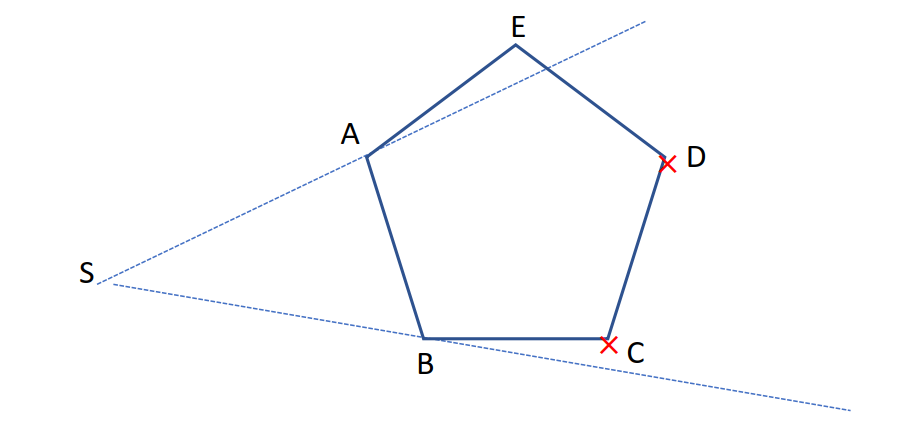
\includegraphics[width=.75\textwidth,height=.75\textheight,keepaspectratio]{can_see.png}
  \caption{Minh hoạ ý tưởng tìm các điểm \textit{nhìn thấy} được từ một đỉnh đến một đa giác}
\end{figure}

Như vậy, từ ý tưởng trên, ta có thể tìm được tất cả các điểm \textit{nhìn thấy} được từ một đỉnh cho trước đến các đa giác lân cận như thuật toán 6 ở bên dưới.

\begin{vnalgorithm}
  \caption{Thuật toán tìm tất cả các điểm \textit{nhìn thấy} được}
  \begin{algorithmic}[1]
    \INPUT {Đỉnh $S$ và các đa giác lân cận $O_1, O_2, \dots, O_n$.}
    \OUTPUT {Tập hợp $V_{see}$ các đỉnh nhìn thấy được.}
    \STATE {$V = $ tập hợp tất cả các đỉnh của các đa giác $O_1, O_2, \dots, O_n$.}
    \STATE {$E = $ tập hợp tất cả các cạnh của các đa giác $O_1, O_2, \dots, O_n$.}
    \STATE {$V_{see} = \emptyset$}
    \FOR {\textbf{each} cạnh $AB$ trong $E$}
      \STATE {$d_1 = $ đường thẳng đi qua $S$ và $A$.}
      \STATE {$d_2 = $ đường thẳng đi qua $S$ và $B$.}
      \STATE {$d_3 = $ đường thẳng đi qua $A$ và $B$.}
      \FOR {\textbf{each} đỉnh $Q \in V\setminus \{S, A, B\}$}
        \IF{$(Q$ và $B$ nằm cùng phía với $d_1) \, \land \, (Q$ và $A$ nằm cùng phía với $d_2) \, \land \, (Q$ và $S$ nằm khác phía với $d_3)$}
          \STATE {$Q$ là đỉnh không nhìn thấy được từ $P$.}
        \ELSE
          \STATE {$Q$ là đỉnh nhìn thấy được từ $P$.}
          \STATE {$V_{see} = V_{see} \cup \{Q\}$}
        \ENDIF
      \ENDFOR
    \ENDFOR
  \end{algorithmic}
\end{vnalgorithm}

\subsection{Hiệu chỉnh thuật toán.}

Một vấn đề của thuật toán trên chính là thuật toán trên chỉ giúp ta tìm được những điểm \textit{nhìn thấy} hay có thể đi qua được. Trên thực tế, không phải điểm nào \textit{nhìn thấy} được là có thể \textit{đi qua} được. Một trường hợp như thế được minh hoạ như hình 4. Ta có thể thấy được đỉnh có toạ độ $(31, 11)$ \textit{nhìn thấy} được đỉnh có toạ độ $(34, 3)$, tuy nhiên ta không thể đi từ đỉnh có toạ độ $(31, 11)$ đến đỉnh có toạ độ $(34, 3)$ vì hai đỉnh này là đường chéo của lục giác.

\begin{figure}[h]
  \centering
  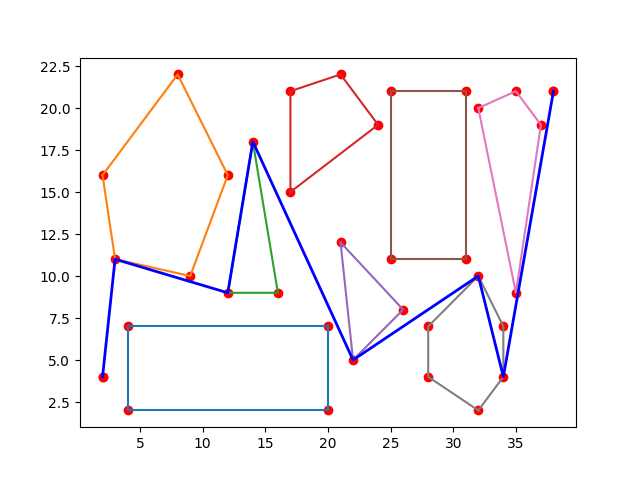
\includegraphics[width=.8\textwidth,height=.8\textheight,keepaspectratio]{not_correct_path.png}
  \caption{Một đường đi không hợp lệ}
\end{figure}

Để có thể giải quyết vấn đề trên, sau khi ta xác định được các điểm nhìn thấy được, ta sẽ loại bỏ đi những đỉnh tạo với đỉnh đang xét một đường chéo của đa giác lân cận, từ đó có thuật toán 7. Kết hợp với các thuật toán tìm kiếm ở trên, ta có thể tiến hành giải quyết bài toán đã cho. Để minh hoạ, ta sẽ giải quyết bài toán trên với đỉnh đầu tiên là đỉnh có toạ độ $(2, 4)$ và đỉnh kết thúc có toạ độ $(38, 21)$.

\begin{vnalgorithm}
  \caption{Thuật toán tìm tất cả các điểm \textit{đi qua} được}
  \begin{algorithmic}[1]
    \INPUT {Đỉnh $S$ và các đa giác lân cận $O_1, O_2, \dots, O_n$.}
    \OUTPUT {Tập hợp $V_{pass}$ các đỉnh có thể đi qua được.}
    \STATE {$V_{see} = $ tập hợp các đỉnh nhìn thấy được từ $S$.}
    \STATE {$V_{pass} = \emptyset$}
    \FOR {\textbf{each} đỉnh $Q \in V_{see}$}
      \IF{$Q$ không nằm trên đường chéo của đa giác lân cận}
        \STATE {$Q$ là đỉnh có thể đi qua được.}
        \STATE {$V_{pass} = V_{pass} \cup \{Q\}$}
      \ENDIF
    \ENDFOR
  \end{algorithmic}
\end{vnalgorithm}

\clearpage

\section{Cài đặt chương trình.}
\subsection{Ghi chú.}
Chương trình sử dụng ngôn ngữ \lstinline|Python| phiên bản 3.9.13, với file đầu vào là \lstinline|input.txt| và mã nguồn được lưu trong file \lstinline|script.py|.

\subsection{Định dạng file đầu vào.}
Dữ liệu của file đầu vào gồm (xem hình 5):
\begin{itemize}
  \item Dòng thứ nhất gồm 5 số nguyên $N, S_x, S_y, G_x, G_y$ cách nhau bởi khỏng trắng, trong đó:
  \begin{itemize}
    \item $N$ là số đa giác nằm trong mặt phẳng $(0 \leq N \leq 100)$.
    \item $(S_x, S_y)$ là toạ độ đỉnh xuất phát.
    \item $(G_x, G_y)$ là toạ độ đỉnh kết thúc.
  \end{itemize}
  \item $N$ dòng tiếp theo gồm các số nguyên $M, X_1, Y_1, \cdots, X_M, Y_M$ cách nhau bởi khỏng trắng, trong đó:
  \begin{itemize}
    \item $M$ là số đỉnh của đa giác.
    \item $(X_i, Y_i)$ là toạ độ thực của đỉnh thứ $i$ trong đa giác.
  \end{itemize}
\end{itemize}

\begin{figure}[h]
  \centering
  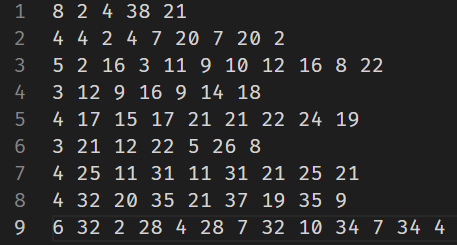
\includegraphics[width=.75\textwidth,height=.75\textheight,keepaspectratio]{input.png}
  \caption{Định dạng file đầu vào \lstinline|input.txt|.}
\end{figure}

\subsection{Các lớp và hàm.}
\subsubsection{Lớp \lstinline|Point|.}
Lớp \lstinline|Point| dùng để định nghĩa một điểm trong không gian trạng thái của bài toán, gồm một số hàm qaun trọng sau:

\begin{itemize}
  \item \lstinline|__init__(self, x, y, polygon_id=-1)|: Khởi tạo những thuộc tính của một điểm, bao gồm hoành độ, tung độ và đa giác mà đỉnh đó thuộc về, nếu không nằm trong đa giác nào, \lstinline|polygon_id = -1|. Ngoài ra, hàm còn khởi tạo thêm chi phí ban đầu \lstinline|g = 0| và thuộc tính \lstinline|pre| lưu lại thông tin \lstinline|Point| trước đó trong đường đi tìm kiếm.
  \item \lstinline|rel(self, other, line)|: Xét vị trí tương đối giữa điểm hiện tại với điểm \lstinline|other| so với đường thẳng \lstinline|line|.
  \item \lstinline|can_see(self, other, line)|: Kiểm tra xem từ điểm hiện tại có thể nhìn thấy được điểm \lstinline|other| qua đường thẳng \lstinline|line| hay không.
  \item \lstinline|line_to(self, other)|: Trả về một đối tượng cạnh \lstinline|Edge| (xem mục \textbf{4.3.2}) nối từ điểm hiện tại đến điểm \lstinline|other|.
  \item \lstinline|heuristic(self, other)|: Trả về kết quả hàm \lstinline|euclid_distance(self, other)| (xem mục \textbf{4.3.4}).
\end{itemize}
\subsubsection{Lớp \lstinline|Edge|.}
Lớp \lstinline|Edge| dùng để định nghĩa một cạnh trong không gian trạng thái của bài toán, trong đó có hai hàm quan trọng sau:
\begin{itemize}
  \item \lstinline|__init__(self, point1, point2)|: Khởi tạo những thuộc tính của một cạnh, bao gồm hai đỉnh \lstinline|Point| là \lstinline|point1| và \lstinline|point2|.
  \item \lstinline|get_adjacent(self, point)|: Trả về đỉnh kề với đỉnh hiện tại (hai đỉnh được gọi là kề nhau nếu chúng nối với nhau bởi một cạnh).
\end{itemize}

\subsubsection{Lớp \lstinline|Graph|.}
Lớp \lstinline|Graph| dùng để định nghĩa một đồ thị trong không gian trạng thái của bài toán. Đây cũng là lớp quan trọng nhất của chương trình, trong lớp này chúng ta quan tâm đến các hàm sau:

\begin{itemize}
  \item \lstinline|__init__(self, polygons)|: Khởi tạo đồ thị \lstinline|self.graph| của bài toán, trong đó \lstinline|polygons| là một danh sách các đa giác, mỗi đa giác là một danh sách các điểm \lstinline|Point| được đọc vào từ file \lstinline|input.txt|. Ngoài ra, hàm này còn lưu tập hợp các cạnh \lstinline|self.edges| và các đa giác \lstinline|self.polygons| của đồ thị.
  \item \lstinline|add_point(self, point)|: Thêm đỉnh \lstinline|point| vào đồ thị.
  \item \lstinline|add_edge(self, edge)|: Thêm cạnh \lstinline|edge| vào đồ thị.
  \item \lstinline|get_points(self)|: Trả về danh sách của đồ thị.
  \item \lstinline|get_edges(self)|: Trả về tập hợp các cạnh của đồ thị.
  \item \lstinline|get_polygons(self)|: Trả về tập hợp các đa giác của đồ thị.
  \item \lstinline|get_adjacent_points(self, point)|: Trả về danh sách các đỉnh kề với đỉnh \lstinline|point|.
  \item \lstinline|can_see(self, start)|: Trả về danh sách các điểm \textit{nhìn thấy} được từ đỉnh \lstinline|start|.
  \item \lstinline|can_go(self, start)|: Trả về tập hợp các điểm có thể di chuyển đến từ đỉnh \lstinline|start|.
  \item \lstinline|h(self, point)|: Trả về giá trị hàm heuristic nếu cần sử dụng, ngược lại trả về $-1$.
\end{itemize}

\subsubsection{Các hàm phụ trợ.}
Ngoài các lớp ở trên, để giải quyết bài toán, chúng ta còn cần các hàm sau:
\begin{itemize}
  \item \lstinline|euclid_distance(point1, point2)|: Trả về khoảng cách Euclide giữa hai điểm \lstinline|point1| và \lstinline|point2|. Khoảng cách Euclide giữa hai điểm $A(x_A, y_A)$ và $B(x_B, y_B)$ được tính bằng công thức:
  \begin{equation}
    d_{AB} = \sqrt{(x_A - x_B)^2 + (y_A - y_B)^2}\nonumber
  \end{equation}
  \item \lstinline|bfs(graph, start, goal)|: Trả về đường đi ngắn nhất từ điểm bắt đầu \lstinline|start| đến điểm kêt thúc \lstinline|goal| trong đồ thị \lstinline|graph| bằng thuật toán BFS.
  \item \lstinline|dfs(graph, start, goal)|: Trả về đường đi ngắn nhất từ điểm bắt đầu \lstinline|start| đến điểm kêt thúc \lstinline|goal| trong đồ thị \lstinline|graph| bằng thuật toán DFS.
  \item \lstinline|ucs(graph, start, goal)|: Trả về đường đi ngắn nhất từ điểm bắt đầu \lstinline|start| đến điểm kêt thúc \lstinline|goal| trong đồ thị \lstinline|graph| bằng thuật toán UCS.
  \item \lstinline|search(graph, start, goal, func)|: Trả về đường đi ngắn nhất từ điểm bắt đầu \lstinline|start| đến điểm kêt thúc \lstinline|goal| trong đồ thị \lstinline|graph|, trong đó \lstinline|func| là một trong hai hàm lambda sau:
  \begin{itemize}
    \item \lstinline|greedy = lambda graph, i: graph.h(i)|: Ứng với thuật toán GBFS.
    \item \lstinline|a_star = lambda graph, i: i.g + graph.h(i)|: Ứng với thuật toán A*.
  \end{itemize}
\end{itemize}

\clearpage
\section{Kết quả thu được.}
Lời giải cho bài toán ban đầu được thể hiện trong hình 6.

\begin{figure}[h]
  \centering
  \begin{subfigure}{.3\linewidth}
      \centering
      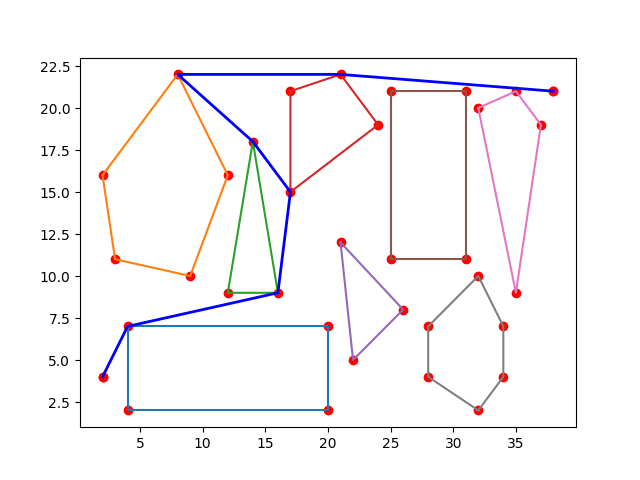
\includegraphics[width=\textwidth,height=\textheight,keepaspectratio]{dfs.png}
      \caption{Thuật toán DFS}
  \end{subfigure}
      \hfill
  \begin{subfigure}{.3\linewidth}
      \centering
      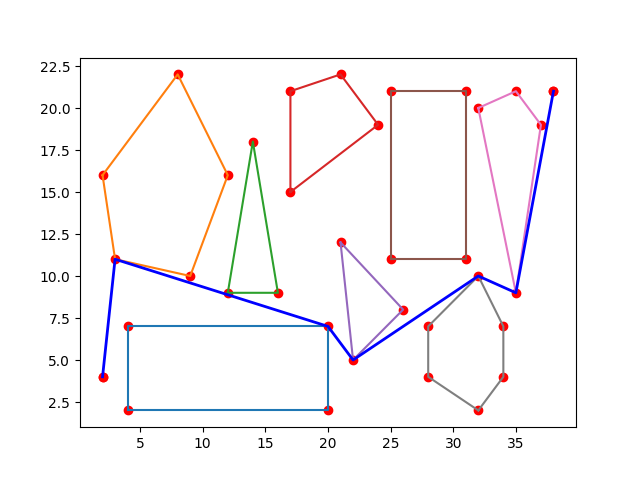
\includegraphics[width=\textwidth,height=\textheight,keepaspectratio]{bfs.png}
      \caption{Thuật toán BFS}
  \end{subfigure}
     \hfill
  \begin{subfigure}{.3\linewidth}
      \centering
      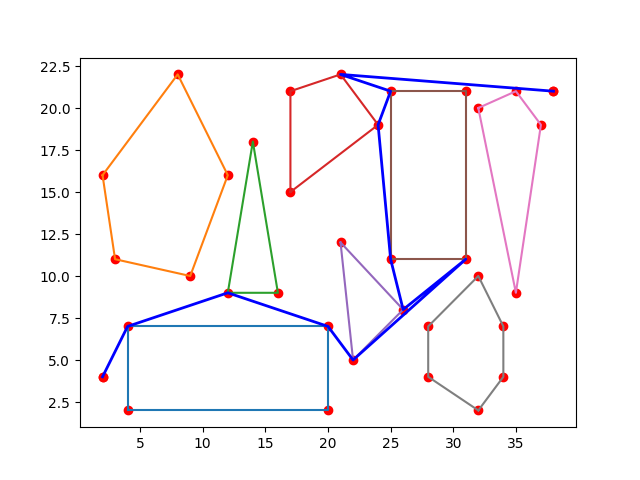
\includegraphics[width=\textwidth,height=\textheight,keepaspectratio]{ucs.png}
      \caption{Thuật toán UCS}
  \end{subfigure}
  
  \bigskip
  \begin{subfigure}{.3\linewidth}
    \centering
    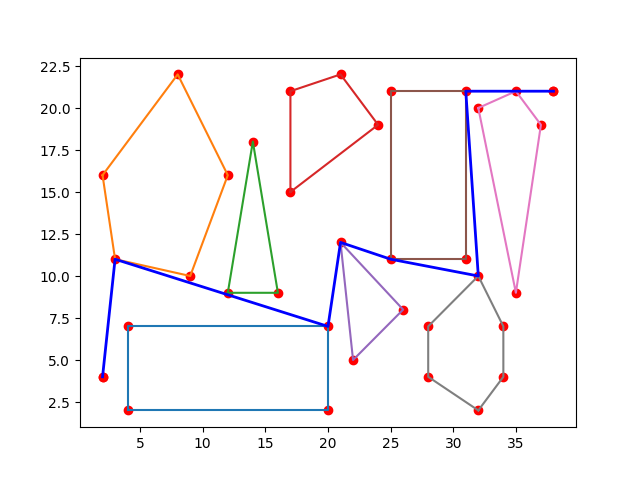
\includegraphics[width=\textwidth,height=\textheight,keepaspectratio]{gbfs.png}
    \caption{Thuật toán GBFS}
  \end{subfigure}
  \hfill
  \begin{subfigure}{.3\linewidth}
    \centering
    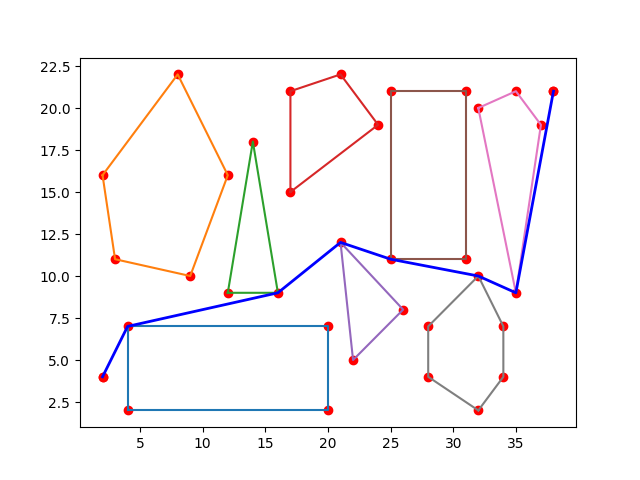
\includegraphics[width=\textwidth,height=\textheight,keepaspectratio]{a_star.png}
    \caption{Thuật toán A*}
  \end{subfigure}
  \caption{Lời giải bài toán ban đầu}
\end{figure}

\section{Nhận xét.}
- Dễ dàng nhận thấy thuật toán A* cho đường đi tốt nhất trong 5 thuật toán tìm kiếm, lý do là bởi thuật toán A* cân bằng giữa chi phí di chuyển và hàm heuristic để tạo ra một đường đi tối ưu nhất có thể.

- Thuật toán UCS cho đường đi không tốt hơn thuật toán BFS và thuật toán DFS. Ta có thề thấy đường đi của thuật toán UCS dài hơn đường đi của thuật toán BFS và thuật toán DFS.

- Thuật toán GBFS cho đường đi tốt hơn thuật toán UCS. Ta có thề thấy đường đi của thuật toán GBFS ngắn hơn nhiều đường đi của thuật toán BFS và thuật toán DFS.

- Mặc dù vậy, cả 5 thuật toán trên vẫn chưa đảm bảo được đường đi tối ưu nhất có thể. Trên thực tế, người ta thường sử dụng một số thuật toán khác để giải quyết bài toán tìm đường đi vượt qua chướng ngại này như là RRT, APF,...


\end{document}